\documentclass{article}
\usepackage[utf8]{inputenc}
\usepackage{amsmath}
\usepackage{amssymb}
\usepackage{cite}
\usepackage{float}
\usepackage{graphicx}
\usepackage{url}

\graphicspath{{./images/}}

\newcommand{\norm}[1]{\left\lVert#1\right\rVert}

\begin{document}

\begin{titlepage}
\begin{center}
\vspace*{1cm}

\Huge
\textbf{Data Assimilation}

\vspace{0.5cm}
\LARGE
Theory and Applications

\vspace{1.5cm}

\textbf{Sebastian Garrido}

\vfill

Supervisor: \\
Dr. Camilo E. Sarmiento

\vspace{0.8cm}


\includegraphics[width=0.4\textwidth]{university}

\Large
Mathematics \\
Universidad del Norte \\
Barranquilla, Atlantico, Colombia \\
November 18, 2018

\end{center}
\end{titlepage}

\section{Introduction}
Correctly modelling physical phenomenon is extremely important as they affect day-to-day operations, e.g. weather has a great influence on traffic. Right now we have the mathematical tools and knowledge to efficiently and accurately predict an wide range of physical occurrences for short windows of time. This is due to the fact that natural systems are usually highly chaotic, and thus, small errors in the initial condition or discrepancies between the model and reality add up such that our predictions tend to diverge from reality after some time. To solve this problem we can use the information from sensors that measure, either directly or indirectly, the system we are making predictions on. Data assimilation is the field which occupies itself with developing techniques that allow integrating information from observations with mathematical models of reality. \\

In this thesis we will introduce a couple of different data assimilation techniques, most of them based on the Kalman Filter, and we will present two concrete applications of statistical filtering, one in the context of Numerical Weather Predictions, and the other in the context Simultaneous Localization and Mapping. \\

\section{Context}

Before giving a rigorous presentation of the Kalman Filter, we would like to give some context on what a filtering problem looks like in reality, and in some way motivate the definitions we will give later on. \\

Imagine the following situation: We have a mathematical model of wind currents in a particular area. We also have a set of wind speed sensors poorly distributed over the area we are modelling. We guess an initial condition for the model and run it for the next 6 hours. We also record measurements made by the wind speed sensors and compare them with the result of our model. We conclude that our model ran somewhat accurately, but would like to introduce some of the information that our sensors recorded into the model. Unfortunately, the sensors we have do not measure the totality of the area we are modelling, and as such, they present an incomplete observation that cannot be directly inserted into the model as an initial condition. Let's assume, just for this exercise, that they also lack information about which direction the wind is headed to. This means that they are an indirect observation, as they don't capture all the kinds of parameters we may be modelling. In a way, if we could represent this data as vectors, we would obtain that they have non-compatible dimensions. Even though these may seem like unsolvable problems, the Kalman Filter allows us to circumvent these issues. \\

\section{Considerations}

From now on, we will assume all vectors are column vectors, except when stated otherwise. \\

We will also assume that the reader is already well-versed in undergraduate level mathematics and computer science. \\

\section{Classical Kalman Filter}

Assume a mathematical model $\mathbf{M}$ of a physical system, a current state of that system $x^b \in \mathbb{R}^m$, an observation $y \in \mathbb{R}^n$, a covariance matrix for the error in the mathematical model $\mathbf{P}^b \in \mathbb{R}^{m \times m}$, a covariance matrix for the error in the observation $\mathbf{R} \in \mathbb{R}^{m \times m}$, and a linear mapping from the space of the model to the space of observations $\mathbf{H} \in \mathbb{R}^{n \times m}$ (also known as the observation operator). If $x^a \in \mathbb{R}^m$ represents the model state after integrating the observations, and $\mathbf{P}^a \in \mathbb{R}^{m \times m}$ represents the model covariance after integrating the observations, then the Kalman Filter equations \cite{Mandel2009} that allow us to find these values are:

\begin{gather*}
x^a = x^b + \mathbf{K} (y - \mathbf{H} x^b) \\
\mathbf{P}^a = (\mathbf{I} - \mathbf{K} \mathbf{H}) \mathbf{P}^b \\
\end{gather*}

where $\mathbf{I}$ represents a compatible identity matrix and $\mathbf{K}$, known as the Kalman Gain, is defined as:

\begin{gather*}
\mathbf{K} = \mathbf{P}^b \mathbf{H}^T (\mathbf{R} + \mathbf{H} \mathbf{P}^b \mathbf{H}^T) ^ {-1} \\
\end{gather*}

Note that the $b$ superscript represents the background, or initial, phase, while the $a$ superscript represents the analysis, or final, phase of the filtering procedure. Also note that the physical system is not used in the Kalman Filter (KF) equations. Presenting it in this section is intentional, as it will become more important later on. \\

\section{Proof of the Classical Kalman Filter}

Assume all errors in the following proof are normally distributed with zero mean, that all covariance matrices are symmetrical, and that the observation operator is orthogonal. Assuming that $x^*$ is the real model state, then the model background state and the observation are sampled as:

\begin{gather*}
x^b \thicksim \mathcal{N}(x^*, \mathbf{P}^b) \\
y \thicksim \mathcal{N}(\mathbf{H} x^*, \mathbf{R}) \\
\end{gather*}

Then, maximum likelihood estimation gives us the following expression:

\begin{gather*}
\frac{1}{\sqrt{(2 \pi)^m |\mathbf{P}^b|}} e^{- \frac{1}{2} (x^b - x^*)^T (\mathbf{P}^b)^{-1} (x^b - x^*)} \cdot \frac{1}{\sqrt{(2 \pi)^n |\mathbf{R}|}} e^{- \frac{1}{2} (y - \mathbf{H} x^*)^T \mathbf{R}^{-1} (y - \mathbf{H} x^*)} \\
\end{gather*}

which can be simplified to:

\begin{gather*}
\frac{1}{\sqrt{(2 \pi)^{m + n} |\mathbf{P}^b| |\mathbf{R}|}} e^{- \frac{1}{2} ((x^b - x^*)^T (\mathbf{P}^b)^{-1} (x^b - x^*) + (y - \mathbf{H} x^*)^T \mathbf{R}^{-1} (y - \mathbf{H} x^*))} \\
\end{gather*}

As we are optimizing with respect to $x^*$ (we need to find the most likely state for our model that could generate both samples), we only need to take into account the variable aspects of the exponent. Therefore, we only need to optimize the following expression:

\begin{gather*}
(x^b - x^*)^T (\mathbf{P}^b)^{-1} (x^b - x^*) + (y - \mathbf{H} x^*)^T \mathbf{R}^{-1} (y - \mathbf{H} x^*) \\
\end{gather*}

To find the optimal value of $x^*$ we derive with respect to it and equate the result to zero. Using matrix-vector derivation properties we arrive at the following expression:

\begin{align*}
&\Rightarrow 0 = -2 \: (x^b - x^*)^T (\mathbf{P}^b)^{-1} - 2 \: (y - \mathbf{H} x^*)^T \mathbf{R}^{-1} \mathbf{H} \\
&\Rightarrow 0 = (x^b - x^*)^T (\mathbf{P}^b)^{-1} + (y - \mathbf{H} x^*)^T \mathbf{R}^{-1} \mathbf{H} \\
&\Rightarrow 0 = (\mathbf{P}^b)^{-T} (x^b - x^*) + \mathbf{H}^T \mathbf{R}^{-T} (y - \mathbf{H} x^*) \\
&\Rightarrow 0 = (\mathbf{P}^b)^{-1} (x^b - x^*) + \mathbf{H}^T \mathbf{R}^{-1} (y - \mathbf{H} x^*) \\
&\Rightarrow (\mathbf{P}^b)^{-1} x^* + \mathbf{H}^T \mathbf{R}^{-1} \mathbf{H} x^* = (\mathbf{P}^b)^{-1} x^b + \mathbf{H}^T \mathbf{R}^{-1} y \\
&\Rightarrow ((\mathbf{P}^b)^{-1} + \mathbf{H}^T \mathbf{R}^{-1} \mathbf{H}) x^* = (\mathbf{P}^b)^{-1} x^b + \mathbf{H}^T \mathbf{R}^{-1} y \\
&\Rightarrow x^* = ((\mathbf{P}^b)^{-1} + \mathbf{H}^T \mathbf{R}^{-1} \mathbf{H})^{-1} ((\mathbf{P}^b)^{-1} x^b + \mathbf{H}^T \mathbf{R}^{-1} y) \\
&\Rightarrow x^* = ((\mathbf{P}^b)^{-1} + \mathbf{H}^T \mathbf{R}^{-1} \mathbf{H})^{-1} ((\mathbf{P}^b)^{-1} x^b \\
& \: \: \: \: \: \: \: \: \: \: \: \: \: \: \: \: + \mathbf{H}^T \mathbf{R}^{-1} \mathbf{H} x^b - \mathbf{H}^T \mathbf{R}^{-1} \mathbf{H} x^b + \mathbf{H}^T \mathbf{R}^{-1} y) \\
&\Rightarrow x^* = x^b + ((\mathbf{P}^b)^{-1} + \mathbf{H}^T \mathbf{R}^{-1} \mathbf{H})^{-1} (- \mathbf{H}^T \mathbf{R}^{-1} \mathbf{H} x^b + \mathbf{H}^T \mathbf{R}^{-1} y) \\
&\Rightarrow x^* = x^b + ((\mathbf{P}^b)^{-1} + \mathbf{H}^T \mathbf{R}^{-1} \mathbf{H})^{-1} \mathbf{H}^T \mathbf{R}^{-1} (y - \mathbf{H} x^b) \\
&\Rightarrow x^* = x^b + \mathbf{K}^* (y - \mathbf{H} x^b) \\
\end{align*}

where $\mathbf{K}^* := ((\mathbf{P}^b)^{-1} + \mathbf{H}^T \mathbf{R}^{-1} \mathbf{H})^{-1} \mathbf{H}^T \mathbf{R}^{-1}$ is known as the information version of the Kalman Gain. This version of the Kalman Gain will become important during the applications as it allows us to set an initial covariance matrix of infinite magnitude (its inverse will just be the zero matrix), which can reduce some of the guesswork involved when estimating initial parameters. This version of the Kalman Gain is also less sensitive to noise. We will now proceed to derive the usual version of the Kalman Gain by proving that $\mathbf{K}^{-1} \mathbf{K}^* = \mathbf{I}$ and therefore $\mathbf{K} = \mathbf{K}^*$. So:

\begin{align*}
\mathbf{K}^{-1} \mathbf{K}^* &= (\mathbf{H} \mathbf{P}^b \mathbf{H}^T + \mathbf{R}) \mathbf{H} (\mathbf{P}^b)^{-1} ((\mathbf{P}^b)^{-1} + \mathbf{H}^T \mathbf{R}^{-1} \mathbf{H})^{-1} \mathbf{H}^T \mathbf{R}^{-1} \\
&= (\mathbf{H} + \mathbf{R} \mathbf{H} (\mathbf{P}^b)^{-1}) ((\mathbf{P}^b)^{-1} + \mathbf{H}^T \mathbf{R}^{-1} \mathbf{H})^{-1} \mathbf{H}^T \mathbf{R}^{-1} \\
&= [\mathbf{R} \mathbf{H} ((\mathbf{P}^b)^{-1} + \mathbf{H}^T \mathbf{R}^{-1} \mathbf{H}) (\mathbf{H} + \mathbf{R} \mathbf{H} (\mathbf{P}^b)^{-1})^{-1}]^{-1} \\
&= [(\mathbf{R} \mathbf{H} (\mathbf{P}^b)^{-1} + \mathbf{H}) (\mathbf{H} + \mathbf{R} \mathbf{H} (\mathbf{P}^b)^{-1})^{-1}]^{-1} \\
&= [(\mathbf{R} \mathbf{H} (\mathbf{P}^b)^{-1} + \mathbf{H}) (\mathbf{R} \mathbf{H} (\mathbf{P}^b)^{-1} + \mathbf{H})^{-1}]^{-1} \\
&= \mathbf{I}^{-1} \\
&= \mathbf{I} \\
\end{align*}

Let's now derive the covariance matrix for the error in $x^*$, assuming $\mathbf{R}$, $\mathbf{P}^b$, $\mathbf{H}$, and $y$ are constant:

\begin{align*}
\mathbf{P}^* &:= Var[x^*] \\
&= Var[x^b + \mathbf{K}(y - \mathbf{H} x^b)] \\
&= Var[x^b] + Var[\mathbf{K}y] - Var[\mathbf{K} \mathbf{H} x^b] \\
&= \mathbf{P}^b - \mathbf{K} \mathbf{H} \mathbf{P}^b \\
&= (\mathbf{I} - \mathbf{K} \mathbf{H}) \mathbf{P}^b \\
\end{align*}

We finish our proof by setting $x^a := x^*$ and $\mathbf{P}^a = \mathbf{P}^*$. \\

\section{Limitations of the Classical Kalman Filter}

Clearly, the formulation of the Kalman Filters asks for conditions that are not usually present in practice:

\begin{itemize}
\item The observation operator is rarely linear and orthogonal.
\item Physical models are rarely linear.
\item Model and observation are not always well-behaved.
\end{itemize}

There are also the memory and computational issues with the Kalman Filter algorithm. Because most realistic physical models have in the order of $O(10^5)$ or $O(10^6)$ data points, storing complete representations of the covariance matrix $\mathbf{P}^b$ and the observation operator $\mathbf{H}$ is usually unfeasible. Even if we ignore the memory problem, we still have to deal with expensive matrix operations over extremely large matrices. In the next few sections we will introduce some techniques to circumvent these issues and make statistical filtering practical. \\

\section{Extended Kalman Filter (EKF)}

Given a non-linear mathematical model $\mathcal{M}$, and a non-linear observation operator $\mathcal{H}$, the main idea of the EKF \cite{Terejanu} is locally linearize both of them using their first-order approximation. If $\mathbf{J}$ is the jacobian operator, then the EKF reduces both of them, at assimilation time $t$, to:

\begin{gather*}
\mathbf{M} (x) = \mathcal{M} (x_{t - 1}^a) + (\mathbf{J} \mathcal{M}) (x_{t - 1}^a) \cdot (x - x_{t - 1}^a) \\
\mathbf{H} (x) = \mathcal{H} (x_{t - 1}^a) + (\mathbf{J} \mathcal{H}) (x_{t - 1}^a) \cdot (x - x_{t - 1}^a) \\
\end{gather*}

\section{Ensemble Kalman Filter (EnKF)}

To solve the representation problem of $\mathbf{P}^b$ we will estimate it using an ensemble of $N$ members sampled from the distribution $\mathcal{N} (x^b, \mathbf{P}^b)$ \cite{Mandel2009}. We will then apply a modified version of the Kalman Filter over this ensemble, which will produce an analysis ensemble. This new ensemble will allow us to estimate $\mathbf{P}^a$. Specifically, let's assume $x_1^b$, $x_2^b$, ..., $x_N^b$ are the members of the background ensemble (the ones estimating $\mathbf{P}^b$). Also assume that $y_1$, $y_2$, ..., $y_N$ are a set of disturbed observations, sampled from $\mathcal{N} (y, \mathbf{R})$. Now define the following matrices:

\begin{gather*}
\mathbf{X}^b =
\begin{pmatrix}
x_1^b & x_2^b & \dots & x_N^b
\end{pmatrix} \\
\mathbf{Y} =
\begin{pmatrix}
y_1 & y_2 & \dots & y_N
\end{pmatrix} \\
\end{gather*}

Then the equation that allows us to derive the analysis ensemble is:

\begin{align*}
\mathbf{X}^a = \mathbf{X}^b + \mathbf{K} (\mathbf{Y} - \mathbf{H} \mathbf{X}^b) \\
\end{align*}

which is structurally identical to the Kalman Filter for the model state. Both $\mathbf{P}^b$ and $\mathbf{P}^a$ are calculated as the covariance matrix of their respective ensemble, where the ensemble members of the analysis ensemble are the columns of $\mathbf{X}^a$. \\

\section{Limitations of the Ensemble Kalman Filter}

Because $N$ is usually in the order of $O(10^3)$, it is usually much smaller than $m$ and the estimated covariance matrix is therefore rank-deficient \cite{Bannister2017}. This prevents inverting the covariance matrix and also brings with it a host of numerical issues. In a later section we will solve this problem using localization. We will also experience convergence of the ensemble members, which may introduce estimation errors as they may become unrepresentative of the distribution they are meant to represent. This issue will be solved by inflation, which again, will be introduced in a later section. \\

\section{Iterative Application of Statistical Filters}

Before continuing we would like to present an overview of how to apply the Kalman Filter iteratively. In practice we rarely assimilate once during the lifetime of the model run as we usually run models for months or even years, expecting meaningful predictions every few hours. This is achieved by assimilating sensor data as soon as we get it. Assume a given interval between assimilations $\Delta$ (which may be variable). Assume also that the current timestep is $t$. If the result of the $t - 1$ assimilation is $x_{t - 1}^a$ (or $X_{t - 1}^a$ if using EnKF) then we can calculate the current background model state using the (not necessarily linear) model $\mathcal{M}$ by $x_t^b = \mathcal{M} (x_{t - 1}^a)$. If we are using an ensemble of model states, we should propagate each individual member in time to obtain the background matrix for the next timestep. We can then perform the assimilation step to obtain $x_t^a$. This procedure can then be repeated ad-infinitum. In practice, this procedure also results in the model error decreasing substantially over time. Notice that we have left out of this discussion how to obtain the initial model state. The next section will present a way to estimate the initial model state efficiently. In a later section we will also show how it replaced a previous technique due to its lower computational cost and similar qualitative properties. \\

\section{Ensemble Kalman Smoother (EnKS)}

To solve the initial condition problem we will use the Ensemble Kalman Smoother \cite{Bannister2017}. First we need to guess an initial condition $x_0^b \in \mathbb{R}^m$ and initial covariance matrix $\mathbf{P}_0 \in \mathbb{R}^{m \times m}$. Then sample a set of ensemble members $x_{0, 1}^b$, $x_{0, 2}^b$, ... , $x_{0, N}^b$, and propagate each of them $t$ times. This will result in sets of ensemble members $x_{k, 1}^b$, $x_{k, 2}^b$, ... , $x_{k, N}^b$, for $1 \leq k \leq t$. Define:

\begin{gather*}
\mathbf{X}^b =
\begin{pmatrix}
x_{0, 1}^b & x_{0, 2}^b & \dots & x_{0, N}^b \\
x_{1, 1}^b & x_{1, 2}^b & \dots & x_{1, N}^b \\
x_{2, 1}^b & x_{2, 2}^b & \dots & x_{2, N}^b \\
\vdots & \vdots & \ddots & \vdots \\
x_{t, 1}^b & x_{t, 2}^b & \dots & x_{t, N}^b
\end{pmatrix} \\
\end{gather*}

Assume also that we have observations $y_k$, for $0 \leq k \leq t$. For each of them, sample a set of disturbed observations $y_{k, 1}$, $y_{k, 2}$, ... , $y_{k, N}$ and define:

\begin{gather*}
\mathbf{Y} =
\begin{pmatrix}
y_{0, 1} & y_{0, 2} & \dots & y_{0, N} \\
y_{1, 1} & y_{1, 2} & \dots & y_{1, N} \\
y_{2, 1} & y_{2, 2} & \dots & y_{2, N} \\
\vdots & \vdots & \ddots & \vdots \\
y_{t, 1} & y_{t, 2} & \dots & y_{t, N}
\end{pmatrix} \\
\end{gather*}

If $\mathbf{H}_0$, $\mathbf{H}_1$, ... , $\mathbf{H}_t$ are the observation operators for each timestep and $\mathbf{R}_0$, $\mathbf{R}_1$, ... , $\mathbf{R}_t$ are the error covariances for each of the observations then define:

\begin{gather*}
\mathbf{H} =
\begin{pmatrix}
H_0 & 0 & \dots & 0 \\
0 & H_1 & \dots & 0 \\
\vdots & \vdots & \ddots & \vdots \\
0 & 0 & \dots & H_t
\end{pmatrix} \\
\\
\mathbf{R} =
\begin{pmatrix}
R_0 & 0 & \dots & 0 \\
0 & R_1 & \dots & 0 \\
\vdots & \vdots & \ddots & \vdots \\
0 & 0 & \dots & R_t
\end{pmatrix} \\
\end{gather*}

Then calculate $\mathbf{X}^a$ using the EnKF equations. Finally, the optimal initial condition is the mean of the column vectors of the submatrix $\mathbf{S} := (\mathbf{X}_{i, j}^a)_{j = 1, 2, ... , N}^{i = 1, 2, ... , m}$. \\

Because the EnKS uses the same equations as the EnKF, it is also possible to reuse existing implementations of the latter when using it. This makes EnKS extremely practical. \\

\section{Localization}

When estimating $\mathbf{P}^b$ from its respective ensemble members, we might obtain spurious correlations between physically unrelated data points in the model due to both numerical issues and the rank-deficiency of the ensemble. For example, assume the following set of differential equations:

\begin{gather*}
\frac{\partial p_i}{\partial t} (t) = p_{(i - 1 \text{ mod } 40)} (t) + p_{(i + 1 \text{ mod } 40)} (t), \: i = 0, 1, ... , 39 \\
\end{gather*}

Because each point is only affected by its neighbours we expect the covariance matrix associated with such model to be banded for a small enough $\Delta$, i.e. to be zero everywhere except in a small band around the main diagonal. In reality, because of the different types of error we describe earlier, the matrix we actually obtain looks somewhat like this:

\begin{figure}[H]
\begin{center}
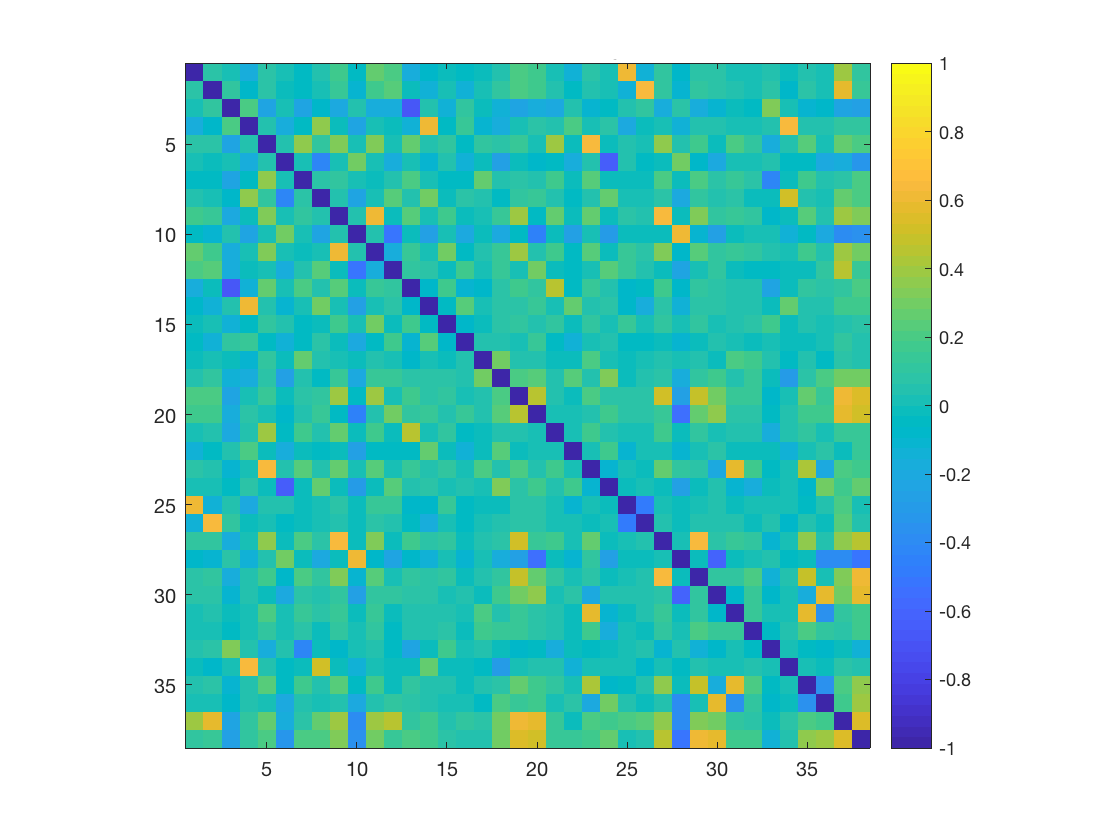
\includegraphics[width=0.8\textwidth]{covariance_before_localization}
\caption{Model error covariance before localization \cite{ROInets}}
\end{center}
\end{figure}

One way to overcome this issue is by using localization. Assume that $\mathbf{P}_l^b$ represents the covariance matrix after localization. Then this matrix can be computed using the Schur (or element-wise) product:

\begin{gather*}
\mathbf{P}_l^b = \rho \circ \mathbf{P}^b \\
\end{gather*}

where $\rho$ can be any compatible matrix, but is usually \cite{Bannister2017}:

\begin{gather*}
(\rho_{0,1})_{i, j} :=
\left\{
\begin{array}{ll}
1 & \mbox{if } d(i, j) \leq d_\text{max} \\
0 & \mbox{otherwise}
\end{array}
\right. \\
\end{gather*}

for some $d_\text{max} \in \mathbb{N}$. In general, $\rho$ should have the form $(\rho)_{i, j} := c(i, j)$, where $c$ is a moderation function that satisfies $c(i, j) = 1$ when $i = j$ and $c(i, j) \rightarrow 0$ when $|i - j| \rightarrow \infty$. The intuition behind these choices is that elements that are separated by enough distance should have a tenuous-at-best relationship. Mathematically, they allow artificially increasing the rank of our covariance matrices.

Continuing with our example, the application of the $\rho_{0,1}$ localization matrix to our example covariance results in:

\begin{figure}[H]
\begin{center}
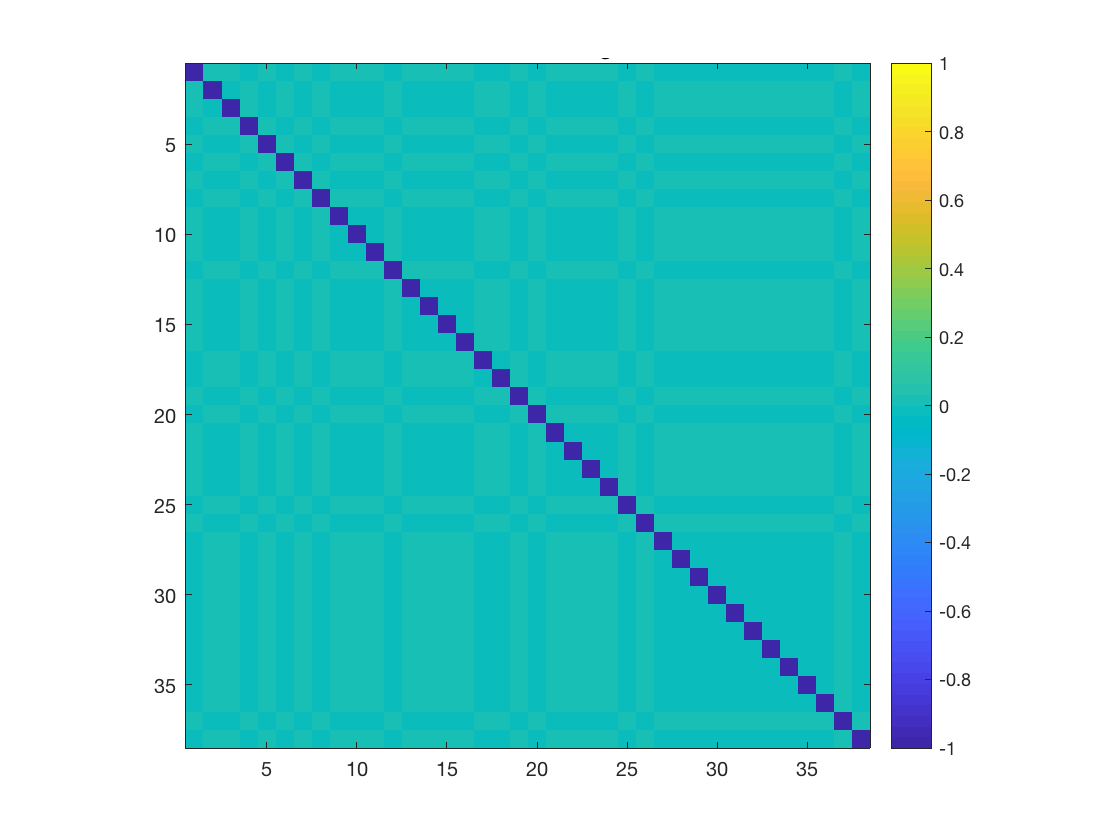
\includegraphics[width=0.8\textwidth]{covariance_after_localization}
\caption{Model error covariance after localization \cite{ROInets}}
\end{center}
\end{figure}

From this example it is clear that $\rho_{0,1}$ is of special interest as it zeroes out elements outside of a certain radius. This allows storing the resulting matrix in a sparse format, which is both memory and computationally efficient. Also, because the resulting matrix is banded we can afford extra optimizations. \\

\section{Inflation}

Iterative application of the filtering algorithm sooner or later produces convergence of our ensemble members. This is undesirable as it is likely that the mean and the covariance matrix associated with this new ensemble will not be representative of the statistical properties of the underlying model error. To solve this problem there are several popular approaches: resampling the ensemble with increased spread, additive/multiplicative inflation \cite{Houtekamer2016}, or square-root filter inflation. The first is self-explanatory, with the inflation parameter obtained experimentally and varying from situation to situation. The second we will not cover due to scope. The final one will be covered in the next section as we cover the square-root type filters. \\

\section{Square Root Filters}

It is common knowledge that population covariance matrices are positive-definite. As such, $\mathbf{P}^a$ ought to be positive-definite. Unfortunately, due to numerical instability in the Kalman Filter, small amounts of noise in the input may affect the sign of the eigenvalues, which would prevent $\mathbf{P}^a$ from being positive-definite after the analysis stage. \\

One solution to this problem is representing $\mathbf{P}^b$ in a way that allows manipulating it without losing the positive-definite property. Using the Cholesky Decomposition helps us obtain the square root $\mathbf{S}^b$ \cite{Tippett2003} of this matrix (which satisfies $\mathbf{P}^b = \mathbf{S}^b (\mathbf{S}^b)^T$). We can now replace $\mathbf{S}^b$ in the Kalman Filter equations and obtain a set of expressions that allows us to obtain the analysis model state $x^a$ and model covariance $\mathbf{S}^a$ in terms of $\mathbf{S}^b$. Finally we can reconstruct $\mathbf{P}^a$ as $\mathbf{S}^a (\mathbf{S}^a)^T$. \\

Another type of square root filter that we will present in a later section is the Local Ensemble Transform Kalman Filter. It uses many of the techniques we have already described which makes it one of the most accurate and efficient data assimilation algorithms to date. It is currently in use in several Numerical Weather Prediction (NWP) centers, as it improved upon the state-of-the-art assimilation quality and computational cost. We will now present some numerical concepts and techniques before introducing this algorithm. \\

\section{Numerical Concepts and Techniques}

\subsection{Spurious Eigenvalues}

Due to numerical factors (approximation, instability, etc.) it is possible finding relatively small eigenvalues that are not related in any way to the physical phenomenon that is being modelled. It is therefore desirable to be able to cancel out or remove these eigenvalues from a matrix as they are mostly noise. SVD Decomposition is one tool that allows us to do just this. \\

\subsection{SVD Decomposition}

Let $\mathbf{A}$ be a real, symmetric, square matrix. Then there are real, orthogonal matrices $\mathbf{U}$ and $\mathbf{V}$, and a diagonal matrix $\mathbf{\Sigma}$ with real non-negative entries such that $\mathbf{A} = \mathbf{U} \mathbf{\Sigma} \mathbf{V}^*$ \cite{CSTheory}. Moreover, the entries of $\mathbf{\Sigma}$ are the eigenvalues of $\mathbf{A}$. They are also usually written from largest to smallest along the principal diagonal. \\

This type of decomposition is extremely useful as it allows us to both observe and directly manipulate the eigenvalues of a matrix. In particular, we will use this technique to remove spurious eigenvalues from the pseudoinverse of a matrix. \\

It is also important to note that the SVD Decomposition can be taken of arbitrary real or complex matrices, but that in the general case the values in the diagonal of $\mathbf{\Sigma}$ are not the eigenvalues but instead the singular values of the matrix $\mathbf{A}$. \\

\subsection{Linear Least Squares}

Given a matrix $\mathbf{A} \in \mathbb{R}^{n \times m}$, and a vector $b \in \mathbb{R}^n$. We would like to find the value of $x \in \mathbb{R}^m$ that minimizes the expression $\norm{\mathbf{A} x - b}$. Clearly, when $\mathbf{A}$ is invertible the solution is $x = \mathbf{A}^{-1} b$. In the more general case it is also possible to find what is known as the pseudoinverse of $\mathbf{A}$, denoted $\mathbf{A}^+$, such that $\mathbf{A}^+ b$ solves the Linear Least Squares problem. In the next subsection we will prove both the existence and unicity of the Moore-Penrose Pseudoinverse, derive its equation and show that it solves the linear least squares problem. \\

\subsection{Pseudoinverse}

The Moore-Penrose Pseudoinverse \cite{CSTheory} of $\mathbf{A} \in \mathbb{R}^{n \times m}$ is defined as the matrix $\mathbf{A}^+ \in \mathbb{R}^{m \times n}$ that satisfies:

\begin{itemize}
\item $\mathbf{A} \mathbf{A}^+ \mathbf{A} = \mathbf{A}$
\item $\mathbf{A}^+ \mathbf{A} \mathbf{A}^+ = \mathbf{A}^+$
\item $(\mathbf{A} \mathbf{A}^+)^* = \mathbf{A} \mathbf{A}^+$
\item $(\mathbf{A}^+ \mathbf{A})^* = \mathbf{A}^+ \mathbf{A}$
\end{itemize}

Let's show that this pseudoinverse is unique. Suppose that for a given matrix $\mathbf{A}$ there are two matrices $\mathbf{B}$ and $\mathbf{C}$ satisfying the required properties. Note that:

\begin{gather*}
\mathbf{A} \mathbf{B} = \mathbf{A} \mathbf{C} \mathbf{A} \mathbf{B} = (\mathbf{A} \mathbf{C})^* (\mathbf{A} \mathbf{B})^* = \mathbf{C}^* \mathbf{A}^* \mathbf{B}^* \mathbf{A}^* = \mathbf{C}^* \mathbf{A}^* = (\mathbf{A} \mathbf{C})^* = \mathbf{A} \mathbf{C} \\
\end{gather*}

Analogously, $\mathbf{B} \mathbf{A} = \mathbf{C} \mathbf{A}$. Then:

\begin{gather*}
\mathbf{B} = \mathbf{B} \mathbf{A} \mathbf{B} = \mathbf{B} \mathbf{A} \mathbf{C} = \mathbf{C} \mathbf{A} \mathbf{C} = \mathbf{C} \\
\end{gather*}

Therefore the Moore-Penrose Pseudoinverse is unique. To show existence let $\mathbf{A}^+ = (\mathbf{A}^* \mathbf{A})^{-1} \mathbf{A}^*$. Then:

\begin{itemize}
\item $\mathbf{A} \mathbf{A}^+ \mathbf{A} = \mathbf{A} (\mathbf{A}^* \mathbf{A})^{-1} \mathbf{A}^* \mathbf{A} = \mathbf{A}$
\item $\mathbf{A}^+ \mathbf{A} \mathbf{A}^+ = (\mathbf{A}^* \mathbf{A})^{-1} \mathbf{A}^* \mathbf{A} \mathbf{A}^+ = \mathbf{A}^+$
\item $(\mathbf{A} \mathbf{A}^+)^* = (\mathbf{A} (\mathbf{A}^* \mathbf{A})^{-1} \mathbf{A}^*)^* = (\mathbf{A} \mathbf{A}^{-1} (\mathbf{A}^*)^{-1} \mathbf{A}^*)^* = \mathbf{I}^* = \mathbf{I} = \mathbf{A} \mathbf{A}^+$
\item $(\mathbf{A}^+ \mathbf{A})^* = ((\mathbf{A}^* \mathbf{A})^{-1} \mathbf{A}^* \mathbf{A})^* = \mathbf{I}^* = \mathbf{I} = (\mathbf{A}^* \mathbf{A})^{-1} \mathbf{A}^* \mathbf{A} = \mathbf{A}^+ \mathbf{A}$
\end{itemize}

which proves existence. To show that $\mathbf{A}^+$ solves the the Linear Least Squares problem, let $z = \mathbf{A}^+ b$ and let $x \in \mathbb{R}^m$. Then:

\begin{align*}
\norm{\mathbf{A} x - b}^2 &= \norm{\mathbf{A} x - b - \mathbf{A} z + \mathbf{A} z}^2 \\
&= \norm{\mathbf{A} (x - z) + \mathbf{A} z - b}^2 \\
&= \norm{\mathbf{A} (x - z)}^2 + (\mathbf{A} (x - z))^* (\mathbf{A} z - b) \\
&\: \: \: \:+ ((\mathbf{A} (x - z))^* (\mathbf{A} z - b))^* + \norm{\mathbf{A} z - b}^2 \\
&= \norm{\mathbf{A} (x - z)}^2 + (x - z)^* \mathbf{A}^* (\mathbf{A} z - b) \\
&\: \: \: \:+ ((x - z)^* \mathbf{A}^* (\mathbf{A} z - b))^* + \norm{\mathbf{A} z - b}^2 \\
\end{align*}

but:

\begin{align*}
\mathbf{A}^* (\mathbf{A} z - b) &= \mathbf{A}^* (\mathbf{A} \mathbf{A}^+ b - b) \\
&= \mathbf{A}^* \mathbf{A} (\mathbf{A}^* \mathbf{A})^{-1} \mathbf{A}^* b - \mathbf{A}^* b \\
&= \mathbf{A}^* b - \mathbf{A}^* b \\
&= 0 \\
\end{align*}

so:

\begin{align*}
\norm{\mathbf{A} x - b}^2 &= \norm{\mathbf{A} (x - z)}^2 + \norm{\mathbf{A} z - b}^2 \\
&\geq \norm{\mathbf{A} z - b}^2 \\
\end{align*}

which proves that the Moore-Penrose Pseudoinverse is a solution to the Linear Least Squares problem. Finally, let's find an expression for the pseudoinverse in terms of the result of SVD decomposition. This will give us the opportunity to manipulate the eigenvalues of a matrix midway through the pseudoinversion process, something which will become useful during the applications. \\

So, if $\mathbf{A} = \mathbf{U} \mathbf{\Sigma} \mathbf{V}^*$, then:

\begin{align*}
\mathbf{A}^+ &= (\mathbf{A}^* \mathbf{A})^{-1} \mathbf{A}^* \\
&= (\mathbf{V} \mathbf{\Sigma}^* \mathbf{U}^* \mathbf{U} \mathbf{\Sigma} \mathbf{V}^*)^{-1} \mathbf{V} \mathbf{\Sigma}^* \mathbf{U}^* \\
&= (\mathbf{V} \mathbf{\Sigma}^*  \mathbf{\Sigma} \mathbf{V}^*)^{-1} \mathbf{V} \mathbf{\Sigma}^* \mathbf{U}^* \\
&= (\mathbf{V} \mathbf{\Sigma} \mathbf{\Sigma} \mathbf{V}^*)^{-1} \mathbf{V} \mathbf{\Sigma} \mathbf{U}^* \\
&= (\mathbf{V} \mathbf{\Sigma}^2 \mathbf{V}^*)^{-1} \mathbf{V} \mathbf{\Sigma} \mathbf{U}^* \\
&= (\mathbf{V}^*)^{-1} \mathbf{\Sigma}^{-2} \mathbf{V}^{-1} \mathbf{V} \mathbf{\Sigma} \mathbf{U}^* \\
&= (\mathbf{V}^*)^{-1} \mathbf{\Sigma}^{-2} \mathbf{\Sigma} \mathbf{U}^* \\
&= \mathbf{V} \mathbf{\Sigma}^{-1} \mathbf{U}^* \\
\end{align*}

\subsection{Domain Decomposition}

Suppose the model state represents a certain quantity over a $k_1 \times k_2 \times \: ... \: \times k_s$ $s$-dimensional grid. If we are using $\rho_{0, 1}$ localization with threshold $d_\text{max}$, we can subdivide the domain into a large number of small grids. Notice that all elements in these small subgrids depend only on themselves plus a small padding around the grid whose size depends on $d_\text{max}$. Because assimilating over these small windows (with a properly-chosen window size) is exponentially faster than assimilating over the full model state we can substantially improve the assimilation speed of our algorithm by performing the assimilation stage over these smaller windows and reconstructing the full analysis by stitching together the results. This also allows massive parallelization of the assimilation algorithm, as each procedure can run fully independent from each other.

\section{Local Ensemble Transform Kalman Filter}

\subsection{Description}

The Local Ensemble Transform Kalman Filter (LETKF) \cite{Hunt2007} is an efficient and stable square root filter, currently in use in many operating NWP centers to perform meteorological data assimilation. Using the square root ensures that we obtain a proper sample mean, that the dependence between members of the ensemble is continuous and thus physically related data points do not diverge too much from each other, and finally, to ensure that analysis perturbations are not so different from background perturbations.

\subsection{Aberration Matrix}

An abberation matrix for a set of column vectors $v_1$, $v_2$, ... , $v_N$ is the matrix:

\begin{gather*}
\begin{pmatrix}
v_1 & v_2 & \dots & v_N
\end{pmatrix} -
\begin{pmatrix}
\bar{v} & \bar{v} & \dots & \bar{v}
\end{pmatrix} \\
\end{gather*}

where $\bar{v}$ is the mean of the collection of vectors $( v_i )_{i = 1, 2, ... , N}$.

\subsection{Algorithm}

Assume an ensemble $x_1^b$, $x_2^b$, ... , $x_N^b$ sampled with covariance $\mathbf{P}^b$. Assume also an observation $y$ with covariance $\mathbf{R}$ and an observation operator $\mathbf{H}$. Assume also an inflation parameter $\sigma$. Finally, assume a $\rho_{0, 1}$ localization matrix with a given threshold $d_\text{max}$. Then the LETKF algorithm is as follows:

\begin{itemize}
\item Let $\bar{y}^b$ be the mean of the collection of vectors $(\mathbf{H} x_i^b)_{i = 1, 2, ... , N}$ and $\mathbf{Y}^b$ be its aberration matrix.
\item Let $\bar{x}^b$ be the mean of the collection of vectors $(x_i^b)_{i = 1, 2, ... , N}$ and $\mathbf{X}^b$ be its aberration matrix.
\item For each data point in the model state do the following:
\item Let $i$ be the current index in the data model.
\item Let $I = \{ j \: | \: \rho_{0, 1} (i, j) = 1 \}$.
\item Let $\mathbf{X}_I^a$ be the submatrix of $\mathbf{X}^a$ which has only the rows indexed by $I$.
\item Let $\mathbf{X}_I^b$ be the submatrix of $\mathbf{X}^b$ which has only the rows indexed by $I$.
\item Let $\mathbf{Y}_I^b$ be the submatrix of $\mathbf{Y}^b$ which has only the rows indexed by $I$.
\item Let $\mathbf{R}_I$ be the submatrix of $\mathbf{R}$ which has only the rows indexed by $I$.
\item Let $\bar{x}_I^b$ be the subvector of $\bar{x}^b$ which has only the rows indexed by $I$.
\item Let $\bar{y}_I^b$ be the subvector of $\bar{y}^b$ which has only the rows indexed by $I$.
\item Let $y_I^b$ be the subvector of $y^b$ which has only the rows indexed by $I$.
\item Let $C = (\mathbf{Y}_I^b)^T \mathbf{R}_I^{-1}$.
\item Let $\tilde{\mathbf{P}^a} = [(N - 1) \mathbf{I} / \sigma + C \mathbf{Y}_I^b]^{-1}$, where $\mathbf{I}$ is a compatible identity matrix.
\item Let $W_1^a = [(N - 1) \tilde{\mathbf{P}^a}]^\frac{1}{2}$.
\item Let $w^a = \tilde{\mathbf{P}^a} (y_I - \bar{y}_I^b)$.
\item Let $W_2^a = W_1^a + ( \: w^a \: w^a \: \dots \: w^a \: )$.
\item Finally set $X_I^a = \bar{x}_I^b + X_I^b W_2^a$ and repeat the previous steps with the next row index. If there are no more rows, then the algorithm has finished executing. Notice that this way we are constructing $X^a$ row-by-row, which is a type of domain decomposition.
\end{itemize}

\section{Application: State-of-the-art Meteorological Data Assimilation}

\subsection{Introduction}

In this section we will introduce a previous state-of-the-art production setup for meteorological data assimilation, show its shortcomings and present a modern setup that addresses these practical issues. Before continuing we must introduce some ideas to understand why the previous setup is less desirable than the current one. \\

\subsection{Automatic Differentiation (AD)}

One often-ignored aspect of differential calculus is that function evaluation and derivative evaluation can be performed side-to-side \cite{ADTheory}. In computational mathematics we are often taught to approximate the derivative using secants. In fact, we can compute the derivative exactly by following a set of rules that are very natural for anyone familiar with derivatives. To do this, we will replace the $x$ value of the function with a tuple $(x, x')$, that follows the following rules:

\begin{itemize}
\item $\text{constant}_c (x, x') = (c, 0)$
\item $(x_1, x_1') + (x_2, x_2') = (x_1 + x_2, x_1' + x_2')$
\item $(x_1, x_1') - (x_2, x_2') = (x_1 - x_2, x_1' - x_2')$
\item $(x_1, x_1') \cdot (x_2, x_2') = (x_1 x_2, x_1' x_2 + x_1 x_2')$
\item $(x_1, x_1') / (x_2, x_2') = (\frac{x_1}{x_2}, \frac{x_1' x_2 - x_1 x_2'}{x_2^2})$
\item $(x, x')^n = (x^n, n (x')^{n - 1})$
\item $\text{sin} (x, x') = (\text{sin} (x), x' \text{cos} (x))$
\item $\text{cos} (x, x') = (\text{cos} (x), - x' \text{sin} (x))$
\item $\text{exp} (x, x') = (\text{exp} (x), x' \text{exp} (x))$
\item $\text{ln} (x, x') = (\text{ln} (x), \frac{x'}{x})$
\item $|(x, x')| = (|x|, x' \text{sign} (x))$
\end{itemize}

In particular, for an initial value of $x_0$, the initial tuple should be $(x_0, 1)$. After simplifying the left side of the tuple will be the function value and the right side will be the value of the derivative at that point. \\

To exemplify let $f(x) = x (e^x + (x + 2) ^ 2)$. Clearly, $f'(x) = (e^x + (x + 2) ^ 2) + x (e^x + 2 (x + 2))$. If $x = 0$ then $f(0) = 0$ and $f'(0) = 5$. Let's prove this:

\begin{align*}
f(0, 1) &= (0, 1) \cdot (\text{exp} (0, 1) + ((0, 1) + (2, 0))^2) \\
&= (0, 1) \cdot (\text{exp} (0, 1) + (2, 1)^2) \\
&= (0, 1) \cdot (\text{exp} (0, 1) + (4, 2)) \\
&= (0, 1) \cdot ((1, 1) + (4, 2)) \\
&= (0, 1) \cdot (5, 3) \\
&= (0, 5) \\
\end{align*}

\subsection{Tangent Linear Model and Adjoint Model}

For a linear model $\mathbf{M}$ its Tangent Linear Model \cite{Benedetti2014} at time $t_i$ is $\mathbf{M}' = \frac{\partial \mathbf{M} [x(t_i)]}{\partial x}$. Its Perturbation Model (to propagate perturbations in time) is $\delta x(t_{i + 1}) = \mathbf{M}' \delta x(t_i)$. The Adjoint Model is defined as $\mathbf{M}^* = (\mathbf{M}')^T$. Let's calculate the Adjoint Model for an example. Assume the following model: \\

\begin{gather*}
z = x + y^2 \\
\end{gather*}

then the Tangent Linear Model is:

\begin{gather*}
\begin{pmatrix}
\delta x \\
\delta y \\
\delta z
\end{pmatrix}
=
\begin{pmatrix}
1 & 0 & 0 \\
0 & 1 & 0 \\
1 & 2z & 0
\end{pmatrix}
\begin{pmatrix}
\delta x \\
\delta y \\
\delta z
\end{pmatrix} \\
\end{gather*}

and the Adjoint Model is:

\begin{gather*}
\begin{pmatrix}
\delta x^* \\
\delta y^* \\
\delta z^*
\end{pmatrix}
=
\begin{pmatrix}
1 & 0 & 1 \\
0 & 1 & 2z \\
0 & 0 & 0
\end{pmatrix}
\begin{pmatrix}
\delta x^* \\
\delta y^* \\
\delta z^*
\end{pmatrix} \\
\end{gather*}

We will now prove the correctness of performing a backwards integration using the adjoint model. This will constitute the main step of the 4D-Var algorithm, which allows us to find an optimal initial condition for our model. Assume a guess for the initial condition of the model $x_0$ and the vectors $x_1$, $x_2$, ... , $x_t$ representing the next $t$ timesteps of our model run. Assume also a background model state $x^b$, and that for each timestep $0 \leq k \leq t$ we have an observation $y_k$, an observation operator $\mathbf{H}_k$, and a covariance matrix for the observation $\mathbf{R}_k$. Finally, assume an initial background model covariance $\mathbf{P}_0^b$. Now define the following cost function:

\begin{gather*}
J(x_0) = \frac{1}{2} (x_0 - x^b)^T (\mathbf{P}_0^b)^{-1} (x_0 - x^b) + \frac{1}{2} \sum_{k = 0}^t (\mathbf{H}_k x_k - y_k)^T \mathbf{R}_k^{-1} (\mathbf{H}_k x_k - y_k) \\
\end{gather*}

Deriving $J$ with respect to the initial condition we get:

\begin{gather*}
\nabla J(x_0) = (\mathbf{P}_0^b)^{-1} (x_0 - x^b) + \sum_{k = 0}^t (\mathbf{M}')_{k \rightarrow 0}^T (\mathbf{H}_k')^T \mathbf{R}_k^{-1} (\mathbf{H}_k' x_k - y_k) \\
\end{gather*}

The main idea now is to study how perturbations in the initial condition affect the cost function. Let $d_k = y_k - \mathbf{H}_k x_k$ and $\delta x_k = \mathbf{M}' \delta x_{k - 1}$ with $\delta x_0 = x_0 - x^b$, for $0 \leq k \leq t$. Substituting into $\nabla J(x_0)$ and using the definition of adjoint model:

\begin{gather*}
\nabla J(\delta x_0) = (\mathbf{P}_0^b)^{-1} \delta x_0 + \sum_{k = 0}^t \mathbf{M}_{k \rightarrow 0}^* \mathbf{H}_k^* \mathbf{R}_k^{-1} (\mathbf{H}_k \delta x_k - d_k) \\
\end{gather*}

or with $\delta x_0 = 0$:

\begin{gather*}
\nabla J(\delta x_0) = - \sum_{k = 0}^t \mathbf{M}_{k \rightarrow 0}^* \mathbf{H}_k^* \mathbf{R}_k^{-1} d_k \\
\end{gather*}

Now let's choose the solution of the adjoint system as follows:

\begin{align*}
x_{t + 1}^*  &= 0 \\
x_0^*  &= \mathbf{M}_1^* x_1^* \\
x_k^*  &= \mathbf{M}_{k + 1}^* x_{k + 1}^* + \mathbf{H}_k^* \mathbf{R}_k^{-1} d_k, \: 1 \leq k \leq t \\
\end{align*}

Progressive substitution on $x_0^*$ results in:

\begin{align*}
x_0^*  &= \mathbf{M}_1^* x_1^* \\
&= \mathbf{M}_1^* (\mathbf{M}_2^* x_2^* + \mathbf{H}_1^* \mathbf{R}_1^{-1} d_1) \\
&= \mathbf{M}_1^* (\mathbf{M}_2^* (\mathbf{M}_3^* x_3^* + \mathbf{H}_2^* \mathbf{R}_2^{-1} d_2) + \mathbf{H}_1^* \mathbf{R}_1^{-1} d_1) \\
&= \: \dots \\
&= \sum_{k = 0}^t \mathbf{M}_1^* \mathbf{M}_2^* \dots \mathbf{M}_k^* \mathbf{H}_k^* \mathbf{R}_k^{-1} d_k \\
&= \sum_{k = 0}^t \mathbf{M}_{k \rightarrow 0}^* \mathbf{H}_k^* \mathbf{R}_k^{-1} d_k \\
&= - \nabla J(\delta x_0) \\
\end{align*}

One idea underlying this proof is that of the interior product. If $<\cdot, \cdot>$ is an interior product, then $<\mathbf{M} x_{t - 1}, x_t> \: = \: <x_{t - 1}, \mathbf{M}^* x_t>$. This implies that in some way the adjoint is integrating the model state back in time, at least when looked through the lens of least-square minimization. \\

\subsection{4D-Var}

The main idea behind this technique is that studying the sensitivity of a model to perturbations in its parameters (initial condition, boundary condition, etc.) allows us to obtain crucial information, like optimal parameters for any given model run \cite{Benedetti2014}. In particular, 4D-Var tries to obtain an optimal initial condition $x_0$ to the model with respect to a set of observations and the results of a model propagation. Empirically, it produces very good results, which has led this technique to be implemented in ECMWF, Meteo France, the Met Office, JMA and CMC, among other NWP centers. \\

To execute 4D-Var perform the following steps:

\begin{itemize}
\item Integrate the model forward from the current initial condition. This will allow us to calculate $J$.
\item Integrate the adjoint model back in time to obtain $\nabla J$.
\item If $\nabla J$ is lower than the tolerance, then our current initial condition is good enough.
\item Otherwise, use $\nabla J$ to estimate a better initial condition using the gradient descent algorithm.
\item If another integration loop is feasible, repeat all the previous steps using the result of the gradient descent algorithm.
\end{itemize}

\subsection{4D-Var Limitations}

Notice that there are several limitations with this approach. First the Tangent Linear Model is obtained by deriving the model and can therefore be calculated using automatic differentiation. In fact, for real-life models with thousands of lines of code this may be the only practical way to find the Tangent Linear Model without risking human error during the derivation. Unfortunately, AD has issues when applied to real-life models. The first one is that it cannot deal with non-differentiable instructions like if statements. AD implementations also tend to generate redundant or memory-inefficient statements which must be cleaned by hand \cite{Giering1998}. \\

There is also the issue that the Tangent Linear Model is at least at expensive to run as the original model, and usually it is 1.5 as expensive. Due to this high cost the optimization loop can rarely be ran more than once or twice, depending on the computational power of the NWP center performing the computation. Another issue is that the model error covariance is assumed to be constant in time, which is rarely the case in practice. The final issue is that the model covariance error is usually too large to represent in memory, as we've stated earlier. \\

In the next section we will present a complete production-ready setup that solves these limitations. \\

\subsection{4D-LETKF}

Given a guess for the initial model state we can efficiently compute an initial state by setting up our integration parameters just like in the EnKS and feeding them into the LETKF. Notice that because the only innovation in the EnKS is in parameter setup, any ensemble filtering algorithm can be turned into a smoother. Given the optimal initial condition we can then use the traditional LETKF to perform iterative filtering on the incoming sensor data. It might also be numerically useful to use the SVD pseudoinverse whenever inversion is non-trivial. \\

Because this method doesn't use the Adjoint Model, we can save ourselves the trouble of coding and computing the model derivative which makes 4D-LETKF substantially more efficient, computation-wise, with respect to 4D-Var. Because 4D-LETKF is an ensemble method, we have also solved the representation problem for $P^b$. Finally, because we can compute $P^b$ from the ensemble members at each timestep, we have solved the model error covariance matrix staticity issue. The only remaining step is to empirically prove the superiority of 4D-LETKF over 4D-Var. \\

\subsection{SPEEDY}

SPEEDY \cite{SPEEDYTheory} (Simplified Parameterizations, privitivE-Equation DYnamics) is a physical weather model that allows us to simulate both local and global phenomenon. It uses an $8$-layered data grid of dimensions $96 \times 48$ which keeps track of vorticity, specific humidity, divergence, absolute temperature, and the natural logarithm of surface pressure (About 184320 data points). It is also extremely efficient, allowing us to run a full-year simulation in 12 minutes using a modest single-core 3.4 GHz computer.

\begin{figure}[H]
\begin{center}
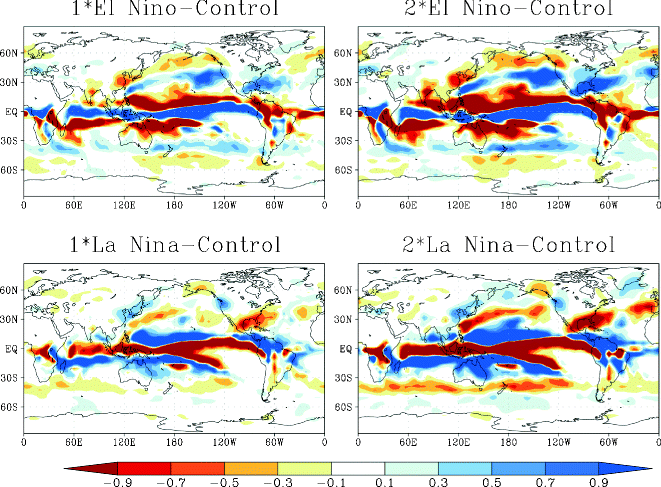
\includegraphics[width=0.8\textwidth]{speedy}
\caption{SPEEDY model run \cite{Dogar2017}}
\end{center}
\end{figure}

\subsection{Experimental Results}

The following graph compares 4D-LETKF with 4D-Var performance during data assimilation in production-like environments. The model used for this experiment was the SPEEDY model we introduced in the previous section. The results clearly show that LETKF is a substantial improvement over 4D-Var in terms of computation time, which adds value to the qualitative improvements we already detailed in the previous subsection.

\begin{figure}[H]
\begin{center}
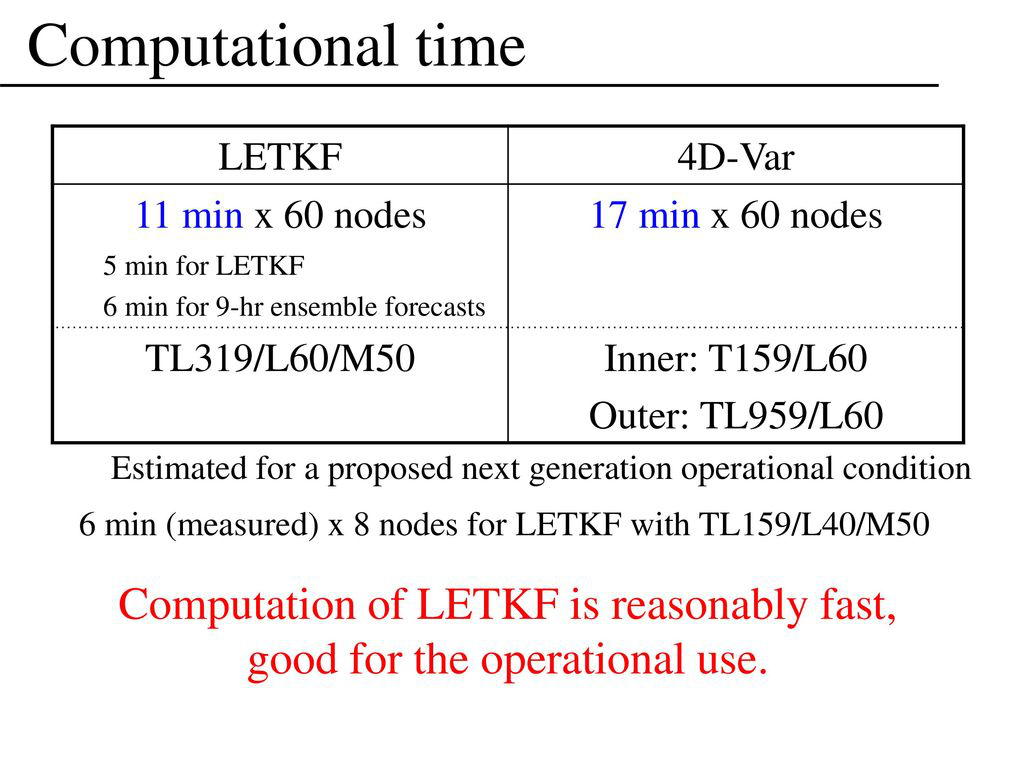
\includegraphics[width=0.8\textwidth]{letkf_vs_4dvar}
\caption{Benchmark results \cite{LETKFJMA}}
\end{center}
\end{figure}

\section{Application: Realtime Simultaneous Localization and Mapping using Monocular Video Sensors}

\subsection{Introduction}

The Simultaneous Localization and Mapping (SLAM) problem is formulated as the problem of determining, given an agent and a set of sensors located at the same position as the agent, the following items:

\begin{itemize}
\item Reconstruction of the map surrounding the agent (Mapping Problem)
\item Locating the agent in the map that is being drawn (Localization Problem)
\item Determining whether a particular location has been visited before by the agent (Loop Closure Problem)
\end{itemize}

There are many applications of SLAM already in consumer electronics. Some of them include self-driving vehicles (e.g. Tesla), autonomous vacuum cleaner (e.g. Roomba) and tracking/recording drones. These applications are usually fed by a wide array of sensors which might include, but are not necessarily limited to, any of the following:

\begin{itemize}
\item Monocular Video
\item Stereo Video
\item Gyroscope
\item Accelerometer
\item Magnetometer
\item LIDAR
\item Motor Feedback
\end{itemize}

Note that all of these sensors, but the first two, provide information about the current position or movement characteristics of the agent in a straightforward fashion. In particular, our application uses only monocular video to perform scaleless SLAM. To add a sense of scale, stereo vision is needed, as the relative position of the cameras with respect to each other encodes all the necessary information to measure objects inside their frame. \\

In this section we will introduce MonoSLAM, the first realtime monocular vision algorithm that solves the SLAM problem. In our exposition we will focus only on the Localization and Mapping problems, even though MonoSLAM solves all of the three problems that make up SLAM. We will now introduce some necessary background: \\

\subsection{Video-based SLAM approaches}

There are two main approaches when it comes to video-based SLAM: sparse and dense strategies. The former attempt to extract meaningful point-features from the image, while the latter attempt to process the full image, obtaining information from areas or patches of the image. Modern dense approaches include LSD-SLAM and DTAM, while moden sparse approaches include Orb-SLAM (v1 and v2), PTAM and MonoSLAM. \\

\begin{figure}[H]
\begin{center}
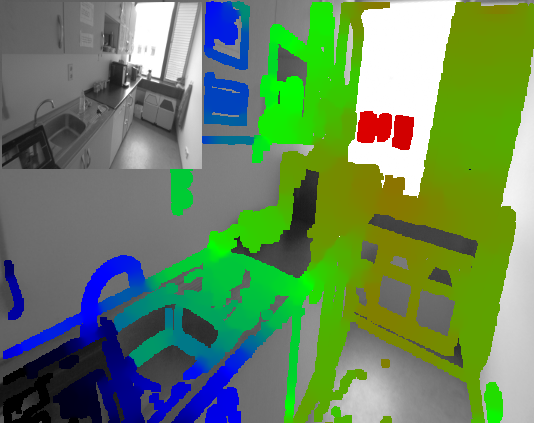
\includegraphics[width=0.4\textwidth]{lsd_slam}
\caption{Dense image processing in LSD-SLAM \cite{engel2013iccv}}
\end{center}
\end{figure}

\begin{figure}[H]
\begin{center}
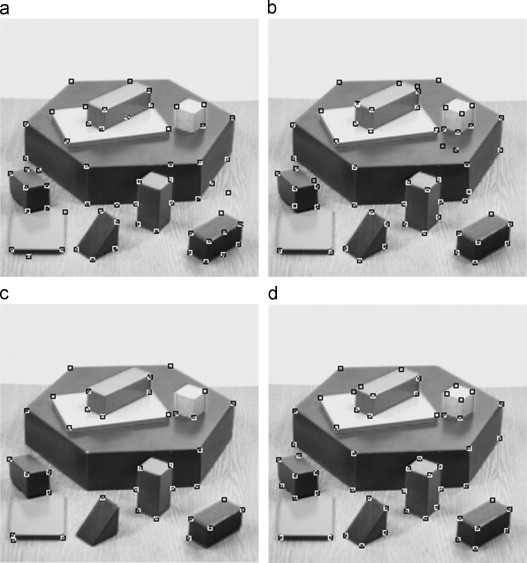
\includegraphics[width=0.4\textwidth]{sparse_image_processing}
\caption{Sparse image processing with Corner Detection \cite{Zhang2015}}
\end{center}
\end{figure}

We will now lay the necessary groundwork behind the video processing capabilities of MonoSLAM. \\

\subsection{Pinhole Camera Model}

Let $(x, y, z) \in \mathbb{R}^3$. Assume a camera with principal point $(u_0, v_0)$, focal length in $x$, $\alpha_x$, focal length in $y$, $\alpha_y$, and skew coefficient $\gamma$. Then the matrix $K$ of intrinsic camera parameters is:

\begin{gather*}
K =
\begin{pmatrix}
\alpha_x & \gamma & u_0 & 0 \\
0 & \alpha_y & v_0 & 0 \\
0 & 0 & 1 & 0
\end{pmatrix} \\
\end{gather*}

Then, given a rotation matrix $R$ and an origin for the world coordinates $T$, we can map this 3D point into 2D space using the pinhole camera model \cite{Hartley2004}:

\begin{gather*}
\begin{pmatrix}
u \\
v \\
1
\end{pmatrix}
=
K[R \: \: \: T]
\begin{pmatrix}
x \\
y \\
z \\
1
\end{pmatrix} \\
\end{gather*}

\subsection{Wide Angle Camera Model}

In the case of a wide angle camera with radial distortion $\theta$, we can define an invertible transformation \cite{Swarninathan1999} that takes into account this distortion. The equations for the wide angle camera model are:

\begin{gather*}
u_d = u_0 + \frac{u - u_0}{\sqrt{1 + 2 \theta r^2}} \\
v_d = v_0 + \frac{v - v_0}{\sqrt{1 + 2 \theta r^2}} \\
\end{gather*}

where $r = \sqrt{(u - u_0)^2 + (v - v_0)^2}$. Wide angle cameras will become particularly useful during MonoSLAM as they have shown better SLAM results experimentally than traditional pinhole cameras. \\

\subsection{Kernel Convolution}

Given a square matrix with odd side-length $\mathbf{G}$ known as the kernel and an arbitrary matrix $\mathbf{A}$, the convolution of $\mathbf{G}$ on $\mathbf{A}$ \cite{EdgeDetection}, noted $\mathbf{G} * \mathbf{A}$ is a matrix with dimension equal to that of $\mathbf{A}$, and whose $(\mathbf{G} * \mathbf{A})_{i, j}$ entry is calculated in the following manner:

\begin{itemize}
\item Let $\mathbf{Q}$ be a window of $\mathbf{A}$ centered on $(i, j)$, with same size as $\mathbf{G}$. For each cell in the window, if the cell extends outside $\mathbf{A}$, set that cell to zero, otherwise set it to the value of $\mathbf{A}$ at that location.
\item Let $\mathbf{Q}' = \mathbf{G} \circ \mathbf{Q}$.
\item Finally, $(\mathbf{G} * \mathbf{A})_{i, j} = \sum_{i, j} \mathbf{Q}'_{i, j}$
\end{itemize}

\subsection{Sobel Operator}

It would be useful to find the "differential of an image", i.e. a measure of how fast an image changes in each pixel. This would allow us to find edges in the image by looking for areas with high rates of change. The Sobel Operator \cite{EdgeDetection} is one possible option to achieve this. Consider the following two matrices:

\begin{gather*}
\mathbf{G}_x
=
\begin{pmatrix}
+1 & 0 & -1 \\
+2 & 0 & -2 \\
+1 & 0 & -1
\end{pmatrix} \\
\\
\mathbf{G}_y
=
\begin{pmatrix}
+1 & +2 & +1 \\
0 & 0 & 0 \\
-1 & -2 & -1
\end{pmatrix} \\
\end{gather*}

Notice that when we apply these matrices using the matrix convolution we defined previously, their form allows us to extract information from the neighbourhood surrounding a pixel. In particular, $\mathbf{G}_x$ computes a measure of change in the x direction, favoring change near the center point while completely ignoring change in the y direction. $\mathbf{G}_y$ behaves analogously but in the y direction instead. We could potentially combine both matrix convolutions to obtain a measure total change:

\begin{gather*}
\mathbf{G} = \sqrt{(\mathbf{G}_x * \mathbf{A})^2 + (\mathbf{G}_y * \mathbf{A})^2} \\
\end{gather*}

This concept of image differential is particularly important when trying to solve the problem of edge detection. Look for example at the application of the Sobel operator to an image: \\

\begin{figure}[H]
\begin{center}
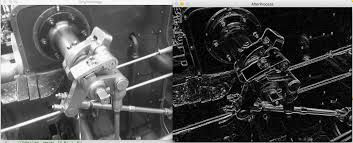
\includegraphics[width=0.8\textwidth]{sobel}
\caption{Sobel operator applied to an Edge Detection Problem}
\end{center}
\end{figure}

It deserves to be noted that images are not matrices, as each pixel in an image has associated with it an RGB value. Because of this we must transform the image to grayscale, which can be represented by a matrix, before calculating the Sobel Operator. \\

\subsection{Shi-Tomasi features}

Edges and specially corners are good feature to track as they tend to change very little from frame to frame during video streams. Shi and Tomasi \cite{JianboShi1994}, following on this idea, derived a feature class from first principles with the intent of making it a good feature to track. This feature is known as a Shi-Tomasi feature. It is computed from an image differential by segmenting the image into windows of small size ($11 \times 11$, $13 \times 13$, and $15 \times 15$ have shown to work well in practice). For each window they compute the Shi-Tomasi operator:

\begin{gather*}
Z
=
\begin{pmatrix}
g_x^2 & g_x g_y \\
g_x g_y & g_y^2
\end{pmatrix} \\
\end{gather*}

where

\begin{gather*}
g_x^2 = \sum_{i, j} (\mathbf{G}_x * \mathbf{A})_{i, j}^2 \\
g_y^2 = \sum_{i, j} (\mathbf{G}_y * \mathbf{A})_{i, j}^2 \\
g_x g_y = \sum_{i, j} (\mathbf{G}_x * \mathbf{A})_{i, j} (\mathbf{G}_y * \mathbf{A})_{i, j}
\end{gather*}

and the sums are over each of the cells of the window. Then the eigenvalues $\lambda_1$ and $\lambda_2$ of $Z$ and we pick $\lambda = \text{min} (\lambda_1, \lambda_2)$. If this lambda is higher than some tolerance value, then we will assume that this window has a Shi-Tomasi feature. Otherwise we will assume that this window has spurious eigenvalues, resulting from numerical errors and should be ignored. \\

\subsection{Particle Filter}

The particle filter \cite{Arulampalam2002} is an algorithm used to estimate arbitrary probability distributions. Intutively, it is also very easy to understand. Assume an initial set of $N$ evenly spaced particles, with each particle having a weight of $\frac{1}{N}$. Then perform a measurement $y$. For each particle, calculate the conditional probability $p(y \: | \: \phi_i)$, for $1 \leq i \leq N$, where $\phi_i$ is the position of the $i$th particle. Then set the new weight of the $i$th particle as $p(y \: | \: \phi_i)$, and normalize the weights of all particles. After a certain number of iterations, the value of the $i$th weight will start to resemble the probability of an observation being sampled with value $\phi_i$. The set of particles will therefore start to look like the probability distribution from where the observations are sampled. \\

The particle filter is extremely useful when we are dealing with non-Gaussian distributions or when we want to test a set of different hypothesis. Unfortunately it requires knowing the conditional probability of observations to some degree of certainty, which will not always be feasible. Luckily, in our application this is not an issue, and therefore, we will ignore this problem for the remainder of the document. \\

\subsection{Mean Shift algorithm}

Assume we have two consecutive frames from the same camera. In the first frame we have an object and a bounding box around the object. In the next frame the object has moved by a small amount and we would like to find the bounding box that most closely matches the shape inside the original image. The mean shift algorithm \cite{Comaniciu2002} solves this problem by creating a "likelihood" image that relates both frames. The mean shift algorithm then takes an initial seed and moves it in the direction of where the "likelihood" image becomes dense, i.e. where similarity between the frames increases. After a number of iterations the seed is guaranteed to converge to a local maximum. This point will be the new center of the bounding box. \\

\subsection{MonoSLAM}

The necessary foundations for MonoSLAM were actually set up years prior to its introduction in the paper \cite{Davison2003}. MonoSLAM was then properly introduced in \cite{Davison2007}. Some work went into it during the next few years, with features like inverse depth parametrization \cite{Civera2008} and scaleless runs being added to the algorithm. \\

MonoSLAM assumes a zero acceleration movement model. This doesn't mean that the algorithm assumes that the agent will never be submitted to acceleration. Instead it assumes that the model to generate background model states never changes the velocity of the agent. This assumption makes sense as for short enough intervals agents will rarely experience acceleration between frames. If a given agent has position vector $r^W$, orientation quaternion $q^{WR}$, velocity vector $v^W$ and angular velocity vector $\omega^W$, then the integration model, for timestep $\Delta t$ is:

\begin{gather*}
\hat{x} =
\begin{pmatrix}
r_\text{new}^W \\
q_\text{new}^{WR} \\
v_\text{new}^W \\
\omega_\text{new}^W
\end{pmatrix}
=
\begin{pmatrix}
r^W + v^W \Delta t \\
q^{WR} \times \mathbf{q}(\omega^W \Delta t) \\
v^W \\
\omega^W
\end{pmatrix} \\
\end{gather*}

Our background model state and covariance are then:

\begin{gather*}
x^b =
\begin{pmatrix}
\hat{x} \\
\hat{y}_1 \\
\hat{y}_2 \\
\vdots
\end{pmatrix} \\
\\
\mathbf{P}^b =
\begin{pmatrix}
\mathbf{P}_{x, x} & \mathbf{P}_{x, y_1} & \mathbf{P}_{x, y_2} & \dots \\
\mathbf{P}_{y_1, x} & \mathbf{P}_{y_1, y_1} & \mathbf{P}_{y_1, y_2} & \dots \\
\mathbf{P}_{y_2, x} & \mathbf{P}_{y_2, y_1} & \mathbf{P}_{y_2, y_2} & \dots \\
\vdots & \vdots & \vdots & \ddots
\end{pmatrix} \\
\end{gather*}

where $\hat{y}_1$, $\hat{y}_2$, ... are the set of image features in 3D space. The set of observations is the result of applying the Mean Shift algorithm to find new 2D positions for each feature. The observation operator is then just the projection of the 3D image features into 2D space using the pinhole camera model (or wide angle, depending on the context). The observation covariance matrix is derived experimentally for the camera being used. \\

Then, a simplified description of the MonoSLAM algorithm is as follows:

\begin{itemize}
\item We wait for an image from the camera.
\item As soon as we get an image we run it through the Sobel Operator.
\item We then calculate the best Shi-Tomasi feature near the principal point of the camera.
\item Using several consecutive images we estimate the position of this feature in the interval going from 0.5 meters to 5 meters using the particle filter. (This estimation can be aided by using previosuly known features with correct depth estimation during the filtering procedure).
\item We then use the Mean Shift algorithm to estimate how much each of the features has moved in the 2D space.
\item We use this information to feed an Extended Kalman Filter that updates the agent's knowledge of itself and its environment
\item We enter into wait mode again.
\end{itemize}

\subsection{Results}

\cite{Davison2007} presents a benchmark for MonoSLAM performance. The author ran the experiments in a 1.6 GHz Pentium M processor, much slower than today's CPUs. He also presented a breakdown of which parts of the algorithm caused which amount of slowdown. Here are the results:

\begin{itemize}
\item Image loading and administration: 2 ms
\item Image correlation searches: 3 ms
\item Kalman Filter update: 5 ms
\item Feature initialization search: 4 ms
\item Graphical rendering: 5 ms
\end{itemize}

for a grand total of 19 ms! This number is much lower than 33 ms, which is the slowest an algorithm that strives to run at 30 frames per second can go. This means that even if a frame takes somewhat longer to process, it is very unlikely that we will still get dropped frames. \\

\bibliography{main}{}
\bibliographystyle{plain}
\end{document}
